\chapter{Caratterizzazione DDS}
Uno dei temi di questa tesi, è stato quello di generare e  analizzare un modello utile per l'implementazione dell'infrastruttura sulla quale tutti gli attori di un Power Stack possano comunicare in modo distribuito. Per poter caratterizzare  l'infrastruttura necessaria, sono stati utilizzati sistemi di High-Performance Computing sui quali andare a testare i vari esperimenti. A supporto di questo lavoro, sono stati resi disponibili due supercalcolatori uno da Cineca\cite{Cineca} e uno da E4\cite{E4} con le specifiche in tabella \ref{table:hpc-cineca}.
%In questo capitolo verranno riportati i casi studio e i test effettuati sul framework. %Tutti questi sono stati eseguiti su un sistema HPC Galileo-100 Cineca con le specifiche riportate nella tabella seguente

\begin{table}[H]
\begin{center}
\begin{tabular}{l|l|l}
    \hline
    \textbf{Parameter} & \textbf{Cineca} & \textbf{E4} \\
    \hline
    Processore & Intel CascadeLake 8260 S & Intel Xeon Silver 4216 \\
    \hline
    [\#] sockets per nodo & 2 & 2 \\
    \hline
    [\#]  core per socket & 24 & 16 \\
    \hline
    Memoria per nodo & 384 GB & 100 GB\\
    \hline
    Connessione & Mellanox Infiniband 100GbE & Eth 100Gb\\
    \hline
    OS & CentOS Linux &  Red Hat Enterprise 8.7\\ 
    \hline
    MPI & Open MPI 4.1.1 & Open MPI 4.1.4 \\
    \hline
\end{tabular}
\end{center}
\caption{Tabella hardware dei sistemi utilizzati}
\label{table:hpc-cineca}
\end{table}

% In tutti i test successivi, ove non specificato diversamente sono stati usati 1 publisher e 48 subscriber su diversi nodi. Questo è stato fatto per provare la scalabilità, visto che nel testbed che è stato utilizzato, erano presenti 48 core (1 core per ogni subscriber).

\section{Strumenti utilizzati}%Struttura dei test
I test effettuati in questa sezione sono stati generati da diversi tipi di componenti ognuno di essi con uno o più compiti specifici, in modo da avere un discreto controllo sull'avanzamento e la gestione dei dati. Nella figura~\ref{fig:schema_global} viene riportato uno schema riassuntivo di tutte le tecnologie utilizzate.
\begin{figure}[H]
    \centering
    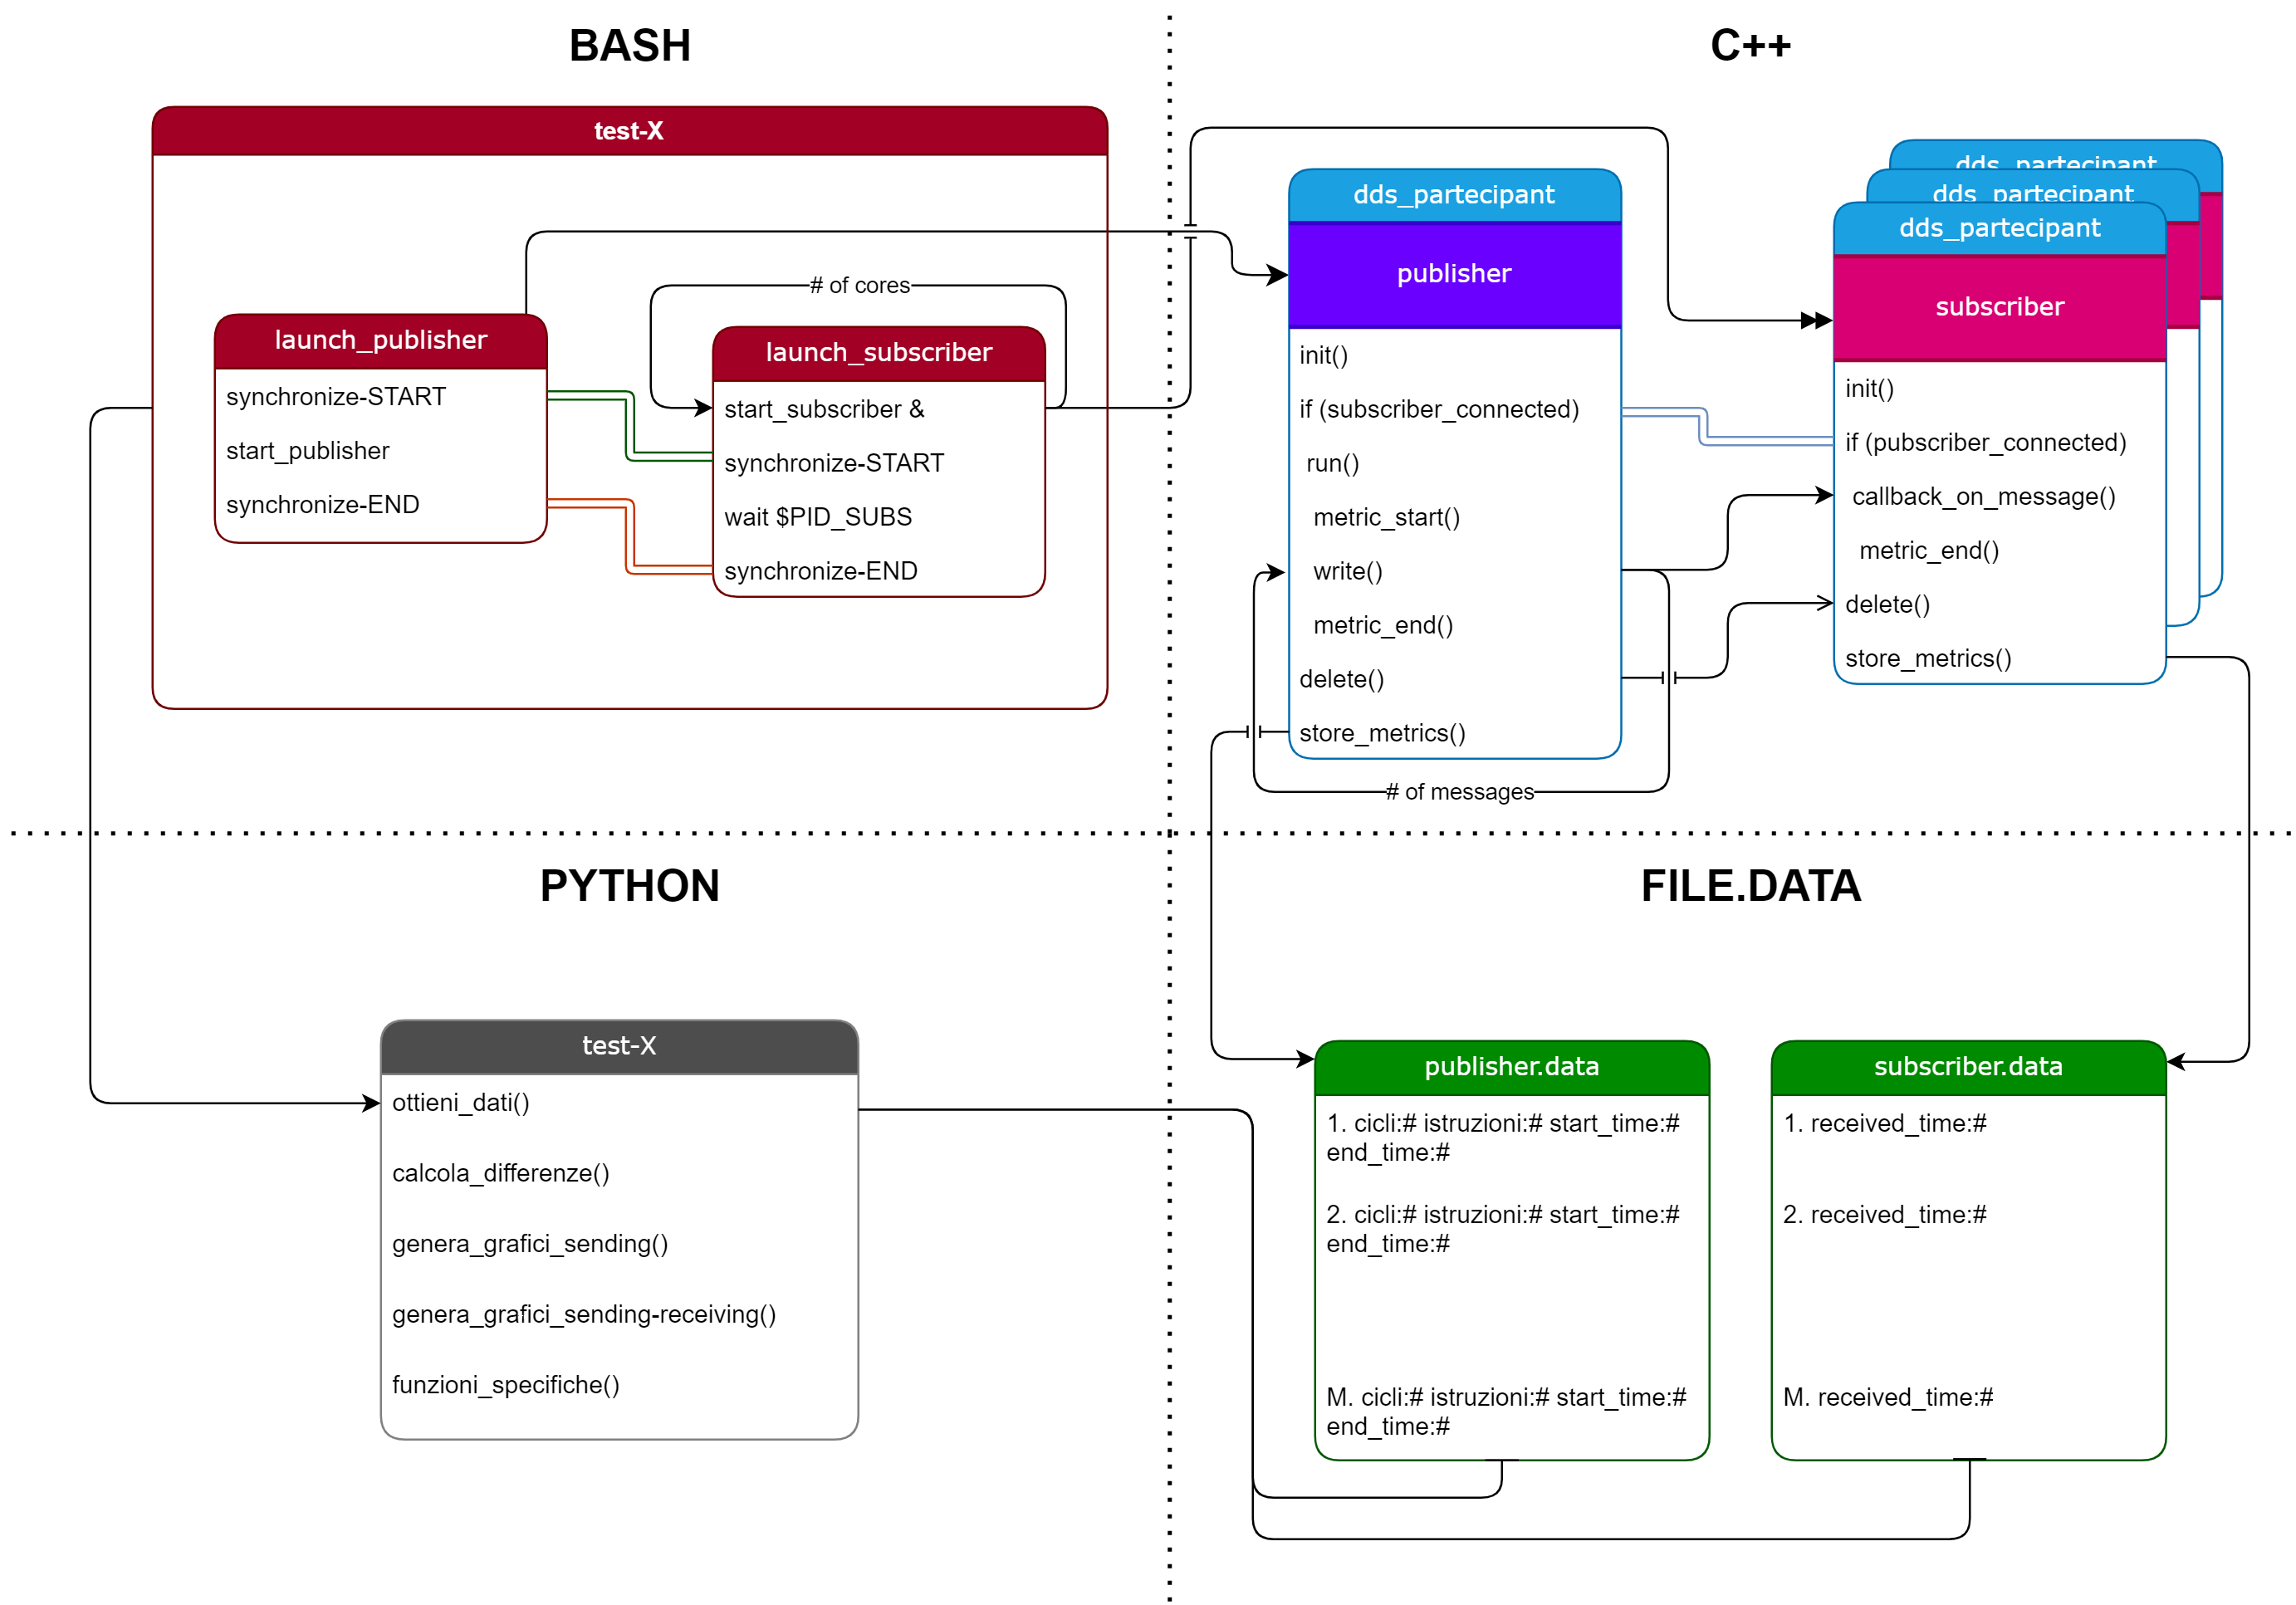
\includegraphics[width=\textwidth]{./img/schema_test_globale.drawio.png}
    \caption{Struttura test}\label{fig:schema_global}
\end{figure}

\subsection{Bash}\label{sec:Shell}
Vista la necessità di lanciare diversi publisher e diversi subscriber ogni volta con dei parametri variabili è stato conveniente usare programmi di scripting come bash. Infatti questi avevano il compito di (i) gestire i diversi parametri da passare agli attori, (ii) inizializzare le variabili d'ambiente, (iii) prendere decisioni di quali core dovevano essere utilizzati da ogni partecipante (task-setaffinity) e (iiii) mantenere sincronizzati i test per evitare che alcuni attori venissero inizializzati troppo presto. Infine ripulivano e ordinavano i dati una volta terminato i test andando ad eseguire gli script python che processavano i dati, nelle cartelle corrette.
\subsection{C++}
E' stato scelto di realizzare una unica versione di publisher e subscriber in cui cambiavano i parametri con cui venivano lanciati. In questo modo è stato più semplice la gestione dei diversi test, e più robusto ad errori dovuti a diverse configurazioni.
\subsubsection*{Struttura}

Per scambiarsi dei messaggi all'interno di infrastruttura basata su DDS, sono necessari: un topic,un publisher ed un subscriber. Inoltre nel topic è necessario definire il tipo dato o struttura di dati che si va a scambiare. La struttura che si è scelta di utilizzare per i test è stata la seguente:
\begin{verbatim}
    struct DDSTest
    {
        unsigned long index;
        std::string message;
    };
\end{verbatim}
Dove index era necessario per definire una corrispondenza stretta tra i messaggi inviati e quelli ricevuti, mentre la stringa era comoda per definire un oggetto di dimensione molto variabile (anche dinamicamente durante i test).
Per quanto concerne al publisher ed al subscriber, sono state utilizzate delle versioni modificate da quelle proposte nella documentazione ufficiale \cite{FastDDS} che andassero sia ad integrare tutte le principali configurazioni possibili, sia integrare alcuni strumenti per l'ottenimento di metriche precedentemente concordate con i collaboratori. Nello specifico sono state scelte per il \textbf{Publisher}:
\begin{itemize}
    \item Tempo di invio;
    \item Istruzioni Perf-Event;
    \item Cicli TSC (read\_tsc);
\end{itemize}
mentre per il \textbf{Subscriber}, solo il tempo di ricezione con un meccanismo di controllo degli indici del messaggio ricevuto.
\subsection{Lettura TSC}
Il Time Stamp Counter, è un registro a 64 bit, presente nella maggior parte dei processori moderni. Il registro fornisce informazioni sul tempo, in termini di cicli di clock del processore, e viene spesso utilizzato per effettuare misure di questo tipo. Il valore, viene letto prima e dopo l'istruzione studiata, tramite l'esecuzione della seguente istruzione:
\begin{verbatim}
    unsigned int lo, hi;
    __asm__ __volatile__ ("rdtsc" : "=a" (lo), "=d" (hi));
    return ((uint64_t)hi << 32) | lo; 
\end{verbatim}
\emph{rdtsc} è l'istruzione assembly per leggere il registro Timestamp Counter, =a (lo) e =d (hi) sono i vincoli di output che specificano come i risultati dell'istruzione rdtsc devono essere restituiti al programma. In lo ("=a") viene riportato il valore a 32 bit meno significativo ed in hi, il valore a 32 bit più significativo.

\subsection{Conteggio istruzioni}
Per le istruzioni invece è stato usato lo strumento \textbf{Perf}, un software offerto da Linux ed incluso anche nel suo kernel, per la profilazione delle performance tramite i \emph{performance\_counter}. Questa suite è estremamente avanzata e permette di ottenere delle metriche a bassa granularità. In questo caso è stata usata una chiamata alla libreria \textbf{perf\_event} utile all'ottenimento del \emph{PERF\_COUNT\_HW\_INSTRUCTIONS}.
\subsection{UML}
Lo schema UML di funzionamento degli attori DDS, con questo approccio, è riassunto e schematizzato dalla figura~\ref{fig:uml}
\begin{figure}[H]
    \centering
    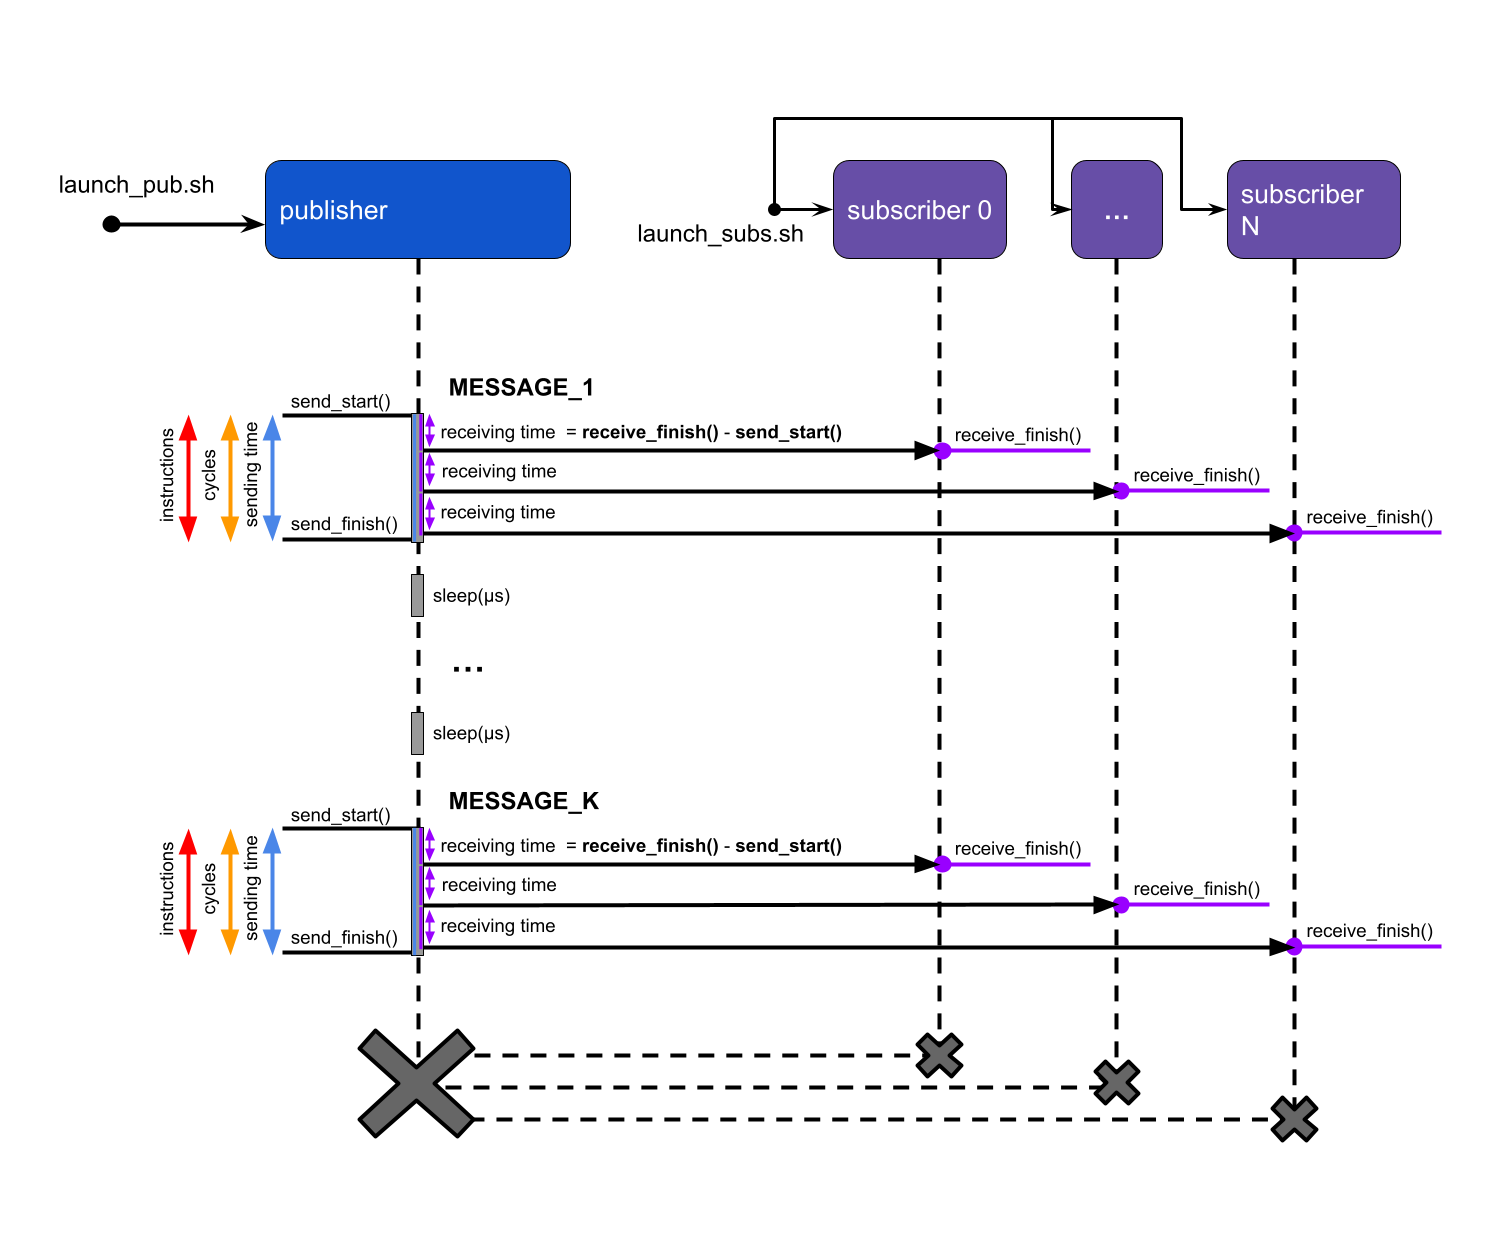
\includegraphics[width=0.9\textwidth]{./img/umel-send-receive.png}
    \caption{Schema UML}\label{fig:uml}
\end{figure}
Come si può vedere, il Publisher~\ref{actor:publisher} prima e dopo la write() salva i valori di tempo di invio, istruzioni, e TSC, mentre al lato ricevente, il Subscriber~\ref{actor:subscriber} salva il tempo di ricezione del messaggio.
\subsection{Ottenimento dei tempi}
In sistemi molto complessi come può essere considerato un supercalcolatore, la gestione degli orologi è tutt'altro che banale. Infatti dopo aver deciso una tra le tante politiche di sincronizzazione disponibile come centralizzata, distribuita e GPS, è necessario continuare a tenere questi orologi aggiornati. Nei sistemi utilizzati in questo progetto, ed in particolare nei supercalcolatori mostrati in tabella~\ref{table:hpc-cineca}, lo strumento adottato è Network Time Protocol (fornito da ntpd). 
Quest'ultimo va a fornire periodicamente agli orologi dei nodi, un tempo di riferimento. Questo intervallo è fissato di default ogni 1024s, ma non disponendo dei diritti necessari, non è stato possibile recuperare questa informazione.

Per ottenere invece le differenze di tempi su sistemi Linux, è ricorrente utilizzare una funzione chiamata \textbf{clock\_gettime()} che restituisce il tempo all'istante della chiamata. Perciò calcolando la differenza tra due diverse clock\_gettime(), si ottiene il tempo trascorso. Il tempo ottenuto, deve avere però un riferimento, non essendo assoluto. Infatti questa funzione mette a disposizione diverse metriche tra cui:
\begin{itemize}
    \item CLOCK\_REALTIME: ottiene il tempo ''reale'' (ore, minuti e secondi del giorno corrente), sincronizzato nei vari sistemi da ntpd;
    \item CLOCK\_MONOTONIC: ottiene un tempo relativo, da un punto non preciso dall'avvio del sistema;
    \item CLOCK\_MONOTONIC\_RAW: ottiene un tempo relativo, da un punto non preciso dall'avvio del sistema, ma non influenzato da ntpd;
    \item CLOCK\_PROCESS\_CPUTIME\_ID: timer dei processori ad alta risoluzione;
    \item CLOCK\_THREAD\_CPUTIME\_ID: tempo dei thread dei processori;
\end{itemize}
Tra tutte queste è stato deciso di utilizzare MONOTONIC, visto che REALTIME con frequenze di aggiornamento di ntpd ogni 1024s fa in tempo ad accumulare sfasamenti di alcuni millisecondi\cite{ntpd}, di gran lunga superiore all'ordine di grandezza da misurare (microsecondi, a volte anche nanosecondi). Inoltre dato che per eseguire i test è stato usato un solo sistema (con più nodi) per volta, la precisione di MONOTONIC\_RAW non è risultata necessaria.

Il problema riscontrato nell'utilizzare  MONOTONIC, è che su sistemi con orologi diversi, questi possono essere sfasati anche di diverse migliaia di secondi. Per aggirare questo problema, sono stati usati 2 approcci completamente diversi:
\begin{itemize}
    \item Sincronizzazione dei nodi
    \item RTT
\end{itemize} 

\subsection{Sincronizzazione}\label{sec:timesync}
Una delle prime soluzioni che è stata provata, è stata quella di sincronizzare gli orologi locali dei diversi nodi tramite l'utilizzo di librerie sviluppate per la programmazione parallela come Message Passing Interface (MPI). Quest'ultimo è un protocollo di comunicazione molto utilizzato nei sistemi HPC per sincronizzare i diversi processi tra di loro.
Nello specifico è stata utilizzata una funzionalità chiamata MPI\_barrier, che permette di bloccare i processi che ne fanno uso,
fino a quando sono tutti sincronizzati, procedendo di conseguenza tutti insieme. Nonostante questo meccanismo fosse particolarmente utile alla sincronizzazione degli orologi non è nato per questo motivo, e racchiudeva per questo alcuni ritardi. Nella figura~\ref{fig:sync_time_shift1} sono stati riportati sull'asse delle Y gli sfasamenti dei tempi di due nodi diversi e sull'asse X il numero dei test effettuati.

\begin{figure}[H]
    \centering
    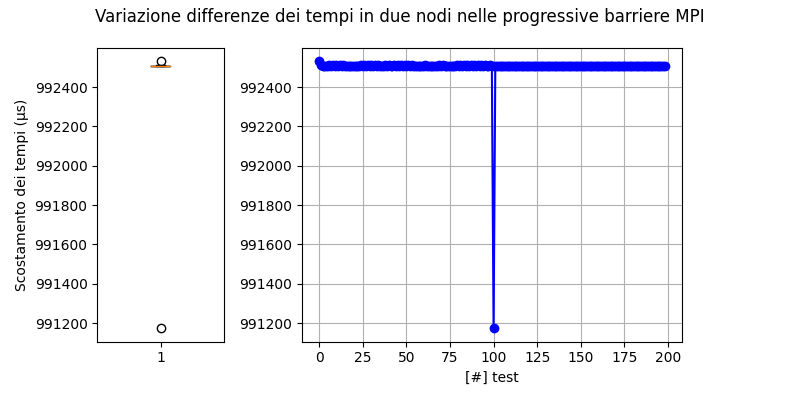
\includegraphics[width=\textwidth]{./results/time_sync_node.png}
    \caption{Scostamento del tempo su nodi diversi}\label{fig:sync_time_shift1}
\end{figure}
% \begin{figure}[H]
%     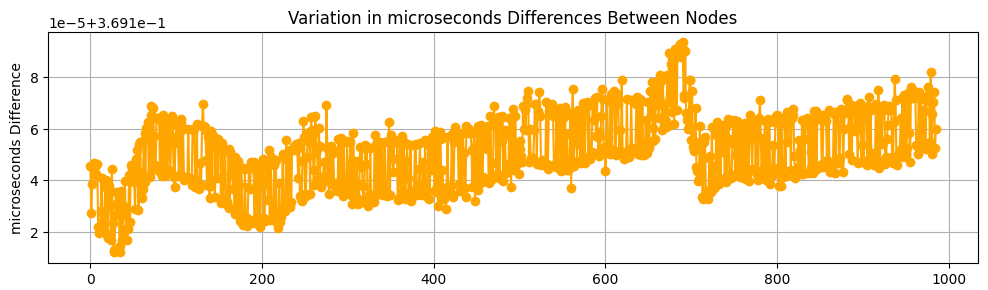
\includegraphics[width=0.99\textwidth]{./results/time_shift_clean.png}
%     \caption{Scostamento senza outliers}\label{fig:sync_time_shift2}
% \end{figure}
% \begin{figure}[H]
%     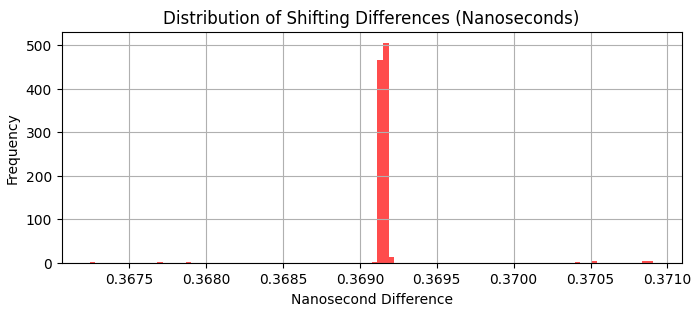
\includegraphics[width=\textwidth]{./results/time_sync_distribution.png}
%     \caption{Distribuzione delle differenze}
%     \label{fig:sync_diff_distr3}
% \end{figure}

Come possibile notare, nonostante le mpi\_barrier, gli scostamenti di tempo tra 2 nodi durante i diversi tentativi effettuati (100), cambia notevolmente, arrivando a differenze fino ad un massimo di 296.659 microsecondi. 
Questo rende il metodo appena mostrato altamente inaffidabile nel 
misurare variazioni di tempi dell'ordine di decine di microsecondi. 


\subsection{RTT}\label{sec:timeRTT}

Nonostante la sincronizzazione fosse idealmente il metodo più preciso per ottenere i tempi di invio-ricezione, essendo l'errore riscontrato, dello stesso ordine di grandezza dei tempi di ricezione, per alcuni test si è utilizzato un approccio che non richiedesse sincronizzazione. Si è scelto quindi di utilizzare il Round Trip Time (RTT).
Questa è un metrica che viene solitamente utilizzata per misurare la latenza di una rete, e si basa sull'idea di calcolare il tempo che intercorre tra l'invio di un segnale e la ricezione della conferma di arrivo dello stesso. Ovviamente il valore ottenuto risulta nel caso ideale più che raddoppiato vista la necessità di un messaggio di risposta. Nel diagramma~\ref{fig:uml} non sarebbe stato possibile condurre questa misura, perchè un subscriber non può inviare un messaggio di risposta.
Per farlo è stato necessario rivedere gli attori coinvolti, ed introdurre in quello che prima venivano chiamati publisher e subscriber, dei meccanismi di ascolto e risposta.
Per semplificarne la comprensione viene riportato lo schema modificato:

\begin{figure}[H]
    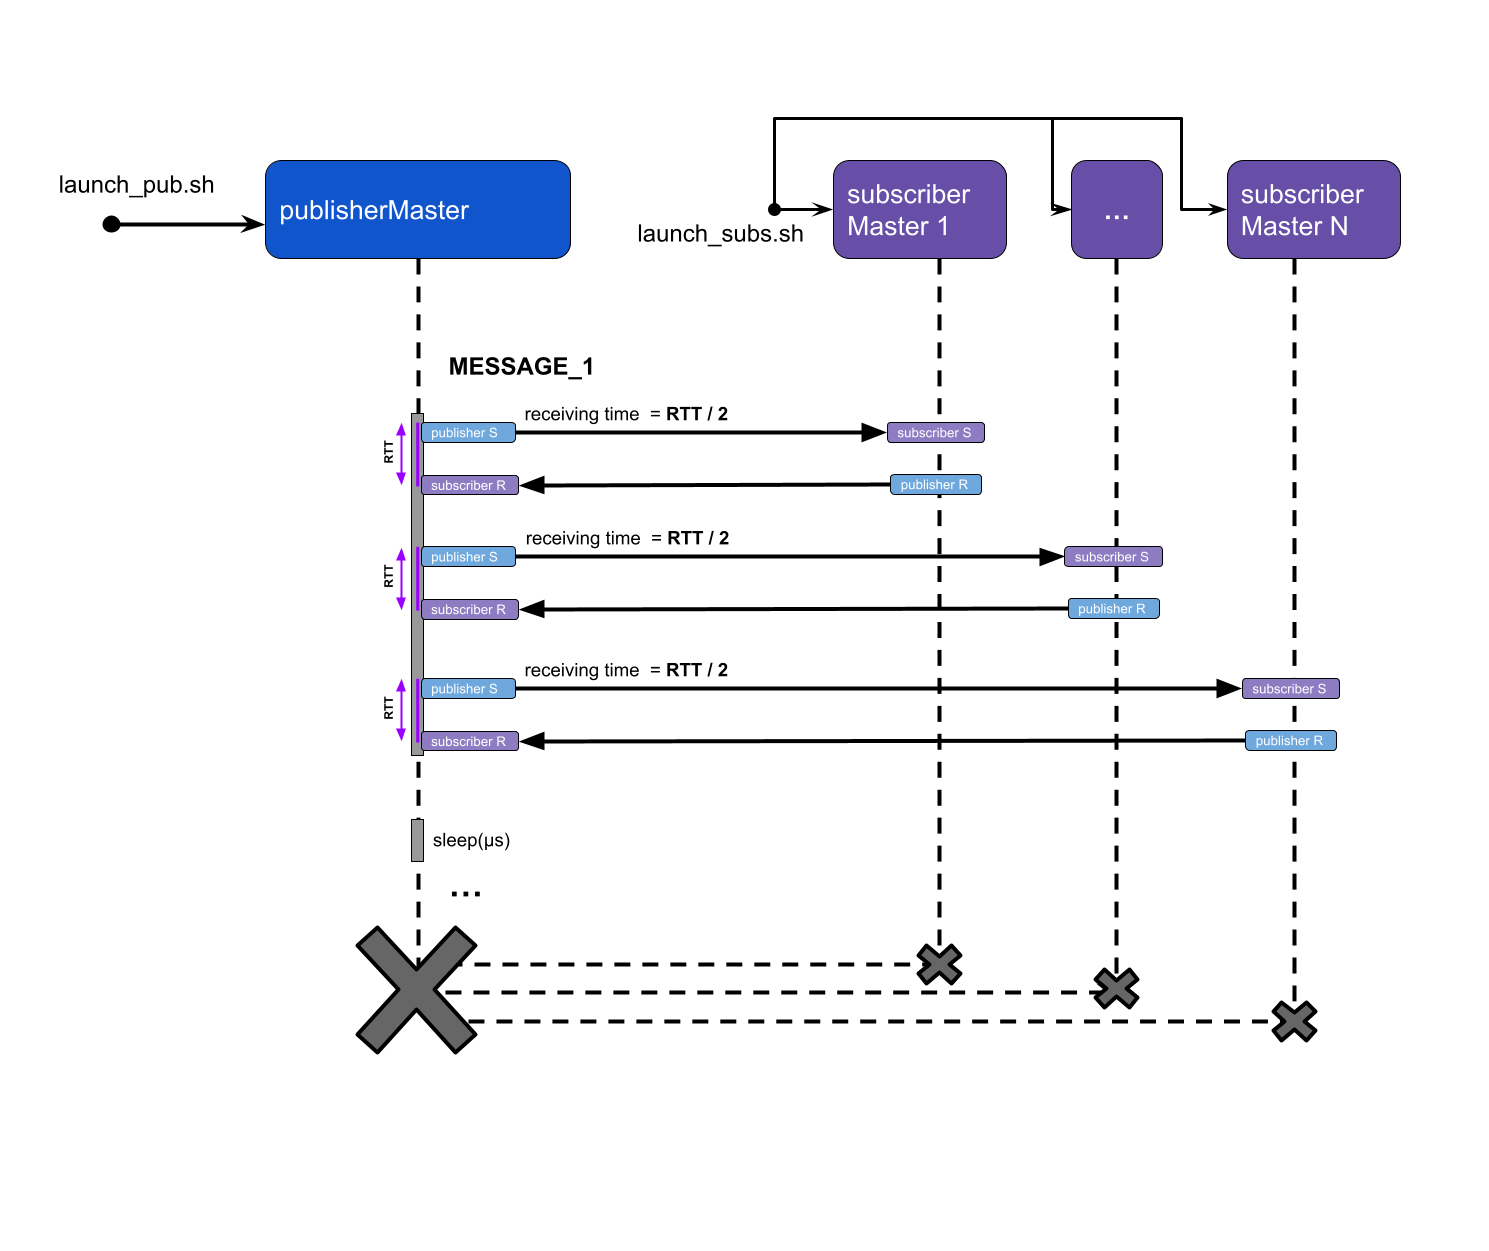
\includegraphics[width=\textwidth]{./img/RTT.png}
    \caption{Schema UML RTT}\label{fig:rtt_uml}
\end{figure} 

Ovviamente questo metodo può comportare qualche ritardo intrinseco di dover gestire due entità per ogni attore, ma sono tempi infinitesimali in confronto al tempo necessario per inviare il messaggio su rete (dove è stato usato questo approccio).

\section{Python}
Gli script python sono stati utili a organizzare e processare tutti i dati oltre a generare tutti i grafici prodotti in questa tesi, considerando che ogni publisher ha generato in ogni test circa 10 mila messaggi, da inviare a tutti e 48 i subscriber, e per ogni protocollo di trasporto, arrivando ad avere per ogni test fino a $1'960'000$ messaggi. 


\section{Schema test}
I test svolti per il modello di utilizzo e per la caratterizzazione di DDS in sistemi HPC sono stati diversi. Nello specifico sono state pensate 4 categorie di test che comprendessero diverse famiglie di problemi:

\begin{itemize}
    \item test-0: discovery
    \item test-1: protocollo di comunicazione
    \item test-2: partizioni e wildcards
    \item test-3: throughput
\end{itemize}

Al fine di condurli nel modo più trasparente possibile sono stati resi disponibili~\cite{mygit} tutti i codici utilizzati durante lo svolgimento di questi test. %TODO5: riordinare & documentare git


\subsection{Discovery}
La prima fase di DDS consiste nel riconoscere altri \emph{dds-partecipant} appartenenti allo stesso dominio. Questa viene chiamata fase di \emph{ Discovery}. Essa ha un ruolo estremamente importante siccome senza non sarebbe possibile far comunicare nessun attore all'interno della stessa rete e nemmeno nello stesso nodo. Una delle peculiarità di DDS è che permette di eseguire tutto in modo completamente distribuito (se non esplicitamente configurato). Il problema sorge, quando si hanno numeri elevati di attori, che per eseguire la discovery (comunicazione due a due), generano migliaia di pacchetti con la conseguente crescita di  computazioni necessarie. %Ovviamente la natura effimera di alcuni di questi componenti potrebbe aggravare il problema. 
Per questo motivo, in DDS sono stati creati dei meccanismi di discovery centralizzati. In questo esperimento si andranno a comparare le due diverse implementazioni e per farlo si useranno gli strumenti \textbf{perf} e \textbf{TCPdump}.
%CONTROLLA CHE SI POSSA FARE TCPDUMP SU CINECA

\subsection{Protocolli di comunicazione}
In DDS ed in particolare nel layer sottostante di RTPS, al fine di scambiare messaggi tramite rete, e non solo nello stesso nodo, è possibile scegliere come mezzo di comunicazione diversi tipi di protocolli:
\begin{itemize}
    \item udp: fornisce la versione v4 e v6 dell'omonimo protocollo di trasporto;
    \item tcp: fornisce la versione v4 e v6 dell'omonimo protocollo di trasporto;
    \item udp-multicast: una versione modificata del semplice udp, dove i subscriber collegati allo stesso topic, hanno un indirizzo comune di ricezione dei dati, permettendo così al publisher di inviare un singolo messaggio che viene condiviso tra tutti;
    \item shared-memory: analogo al metodo precedentemente, ma invece di utilizzare un indirizzo IP, viene utilizzato un indirizzo di memoria. E' possibile solo quando i due processi che comunicano sono sullo stesso nodo, con memoria condivisa;
\end{itemize}

Nel primo test si è valutata la differenza di queste implementazioni utilizzando la rete infiniband~\ref{table:hpc-cineca} sui diversi nodi del supercalcolatore. 

\subsection{Wildcards e metodi di instradamento}
Un concetto fondamentale nelle comunicazioni tra attori con gerarchie diverse, in sistemi con diverse centinaia di migliaia di entita, come cluster, nodi, processori, job (etc.), sono le possibilità di instradare, segmentare e rendere gerarchiche le comunicazioni. Come spiegatolo nel capitolo~\ref{Chapter:dds} in DDS ci sono diversi strumenti disponibili per farlo. Tra di loro differiscono per alcuni aspetti, come flessibilità, costo (in performance) e livello di segmentazione.

\subsubsection{Dominio} 
Il dominio è la segmentazione di più ``forte`` e di più alto livello. Va a partizionare gli attori presenti in un dominio in modo del tutto fisico (cambiando per ogni dominio porte e indirizzi di comunicazione) e per nulla flessibile. Per cambiare il dominio è necessario distruggere e creare di nuovo il partecipante. Inoltre il dominio non permette nessun tipo di gerarchia.
    
\subsubsection{Topic}
All'interno di un dominio, i topic costituiscono la scelta predefinita di instradamento dei messaggi, essendo però limitato dal tipo di messaggio che si vuole inviare. Infatti topic diversi supportano tipi di dato diversi, e non sono modificabili durante il loro utilizzo.
Inoltre il topic non permette gerarchie ed è difficilmente modificabile a run-time.

\subsubsection{Partizione}
Questo strumento risulta molto interessante, in quanto permette di definire gerarchie e wildcards all'interno di un dominio creando una segmentazione virtuale. Inoltre è facilmente modificabile a run-time.

\subsubsection{Wildcards}
Le wildcards sono un costrutto appartenente alle partizioni, che definisce dei pattern testuali sulla base del quale vengono instradati i messaggi. Un esempio può essere \textit{Node*} che va a corrisponde a tutti i messaggi sotto il topic precedentemente definito, a tutte le partizioni che iniziano con Node.

\begin{figure}[H]
    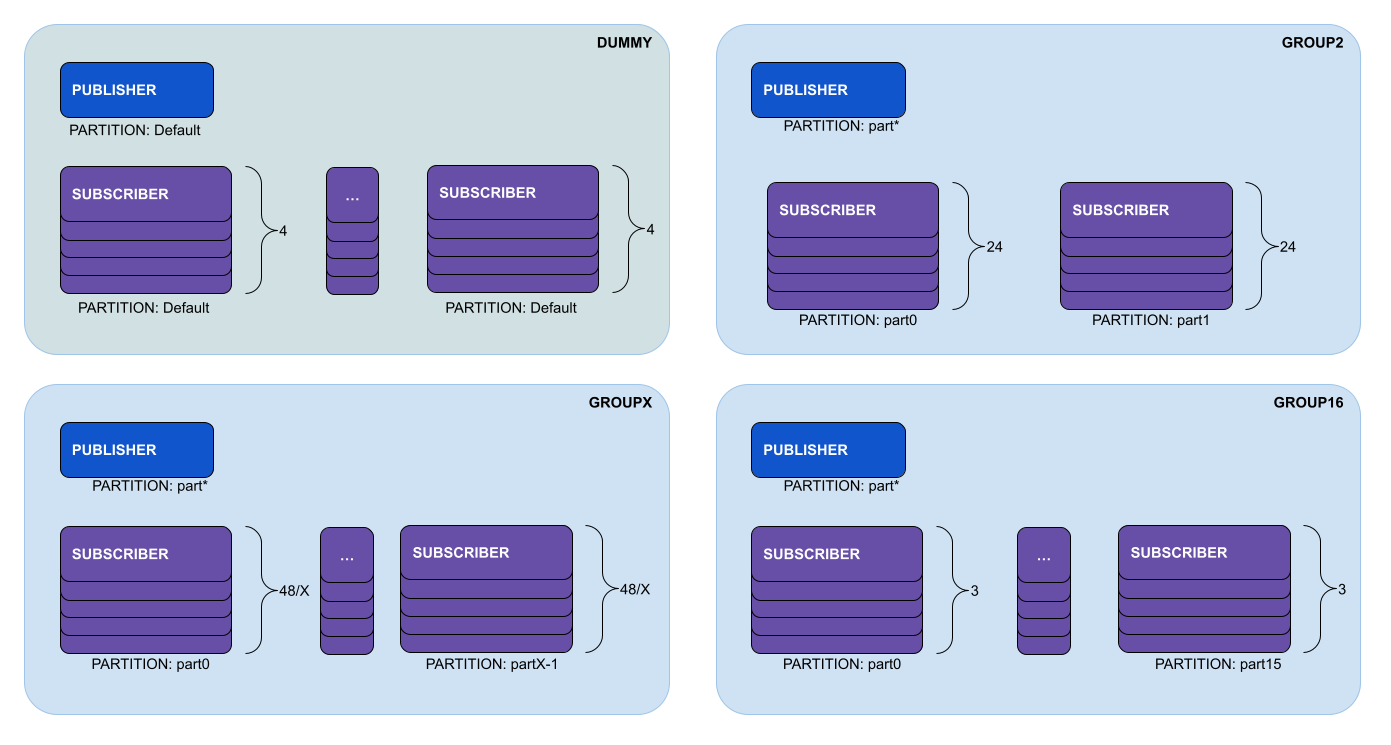
\includegraphics[width=\textwidth]{./img/wildcards.png}
    \caption{Schema test wildcards}\label{fig:test_UML_wildcards}
\end{figure} 

In questo test si è valutata la differenza in termini di performance dei diversi strumenti, con un particolare focus sulle partizioni e le wildcards, con schema in figura~\ref{fig:test_UML_wildcards}.

\subsection{Throughput}
Nell'ultimo esperimento ci si è focalizzati sulla caratterizzazione di questo middleware ed in particolare è stato misurato il throughput e la frequenza di scambio dei messaggi nei sistemi target. 
%, valori particolarmente importanti quando si parla di sistemi con volumi di scambio estremamente elevati. 
Per farlo, sono stati eseguiti i test su tutti e 4 i protocolli messi a disposizione e con volumi di scambio più elevati, al fine di fornire una panoramica completa. %Inoltre per calcolarlo sono usate le configurazioni in tabella~\ref{table:test3} per simulare un carico di comunicazioni elevato tra attori di HPC.\@Nella vengono riportati i parametri scelti.

% \begin{table}[H]
%     \begin{center}
%     \begin{tabular}{l|l}
%         \hline
%         \textbf{Parametri} & \textbf{throughput} \\
%         \hline
%         [\#] publisher & 1  \\
%         \hline
%         [\#] subscriber & 40 \\
%         \hline
%         [\#] messaggi scambiati (per attore) & 10 000 \\
%         \hline
%         Dimensione del messaggio & 16 Byte \\
%         \hline
%     \end{tabular}
%     \end{center}
%     \caption{Valori usati per il test 3}\label{table:test3}
%     \end{table}
    
